\documentclass[letterpaper,headings=standardclasses]{scrartcl}

\usepackage[margin=1in,includefoot]{geometry}
\usepackage{amssymb}
\usepackage{amsmath}
\usepackage{listings}
\usepackage{tikz}
\usepackage{float}

\usetikzlibrary{shapes,arrows}

\tikzset{
  block/.style    = {draw, thick, rectangle, minimum height = 3em, minimum width = 3em},
  sum/.style      = {draw, circle},
  input/.style    = {coordinate, circle},
  output/.style   = {coordinate, circle}
}

\lstset{basicstyle=\ttfamily,language=python,columns=flexible,breaklines=true,showstringspaces=false}

\title{Homework 7}
\subtitle{CS 559 - Neural Networks - Fall 2019}
\author{Matteo Corain 650088272}

\begin{document}

\maketitle

\section{Question 1}

\subsection{Training set generation}

The training set for the SVM to be designed has been generated by randomly selecting $n = 100$ points in $[0,1]^2$ through the \texttt{uniform()} function offered by the NumPy package. The class labels associated to such points has been selected as:

$$ d_i = \begin{cases} +1 & \text{if } x_{i2} < 0.2 \sin{(10x_{i1})} + 0.3 \vee (x_{i2} - 0.8)^2 + (x_{i1} - 0.5)^2 < 0.15^2 \\ -1 & \text{otherwise} \end{cases} $$

The obtained set of points is shown in figure \ref{data}, which is produced by the \texttt{plot\_data()} function. This procedure simply plots the data points and the ``exact'' separator, after having evaluated it on a set of equidistant values in $[0,1]$.

\begin{figure}[h]
    \centering
    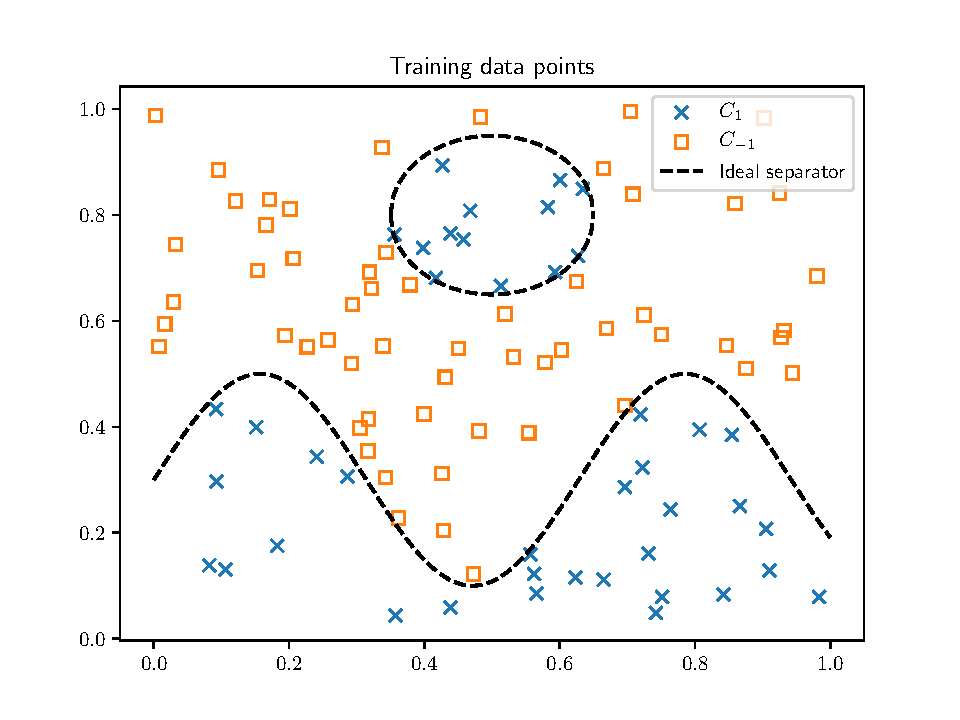
\includegraphics[width=0.7\linewidth]{data.pdf}
    \caption{Data set for the exercise}
    \label{data}
\end{figure}

\subsection{SVM problem formalization}

Let us recall that the SVM problem is to define the values of $\alpha_1, \dots, \alpha_n$ that satisfy the following optimization problem:

$$ \max_{\substack{\alpha_1, \dots, \alpha_n \ge 0 \\ \scriptstyle \sum_{i = 1}^n \alpha_i d_i = 0}}{\left( \sum_{i = 1}^n \alpha_i - \frac{1}{2} \sum_{i = 1}^n \sum_{j = 1}^n \alpha_i \alpha_j d_i d_j K(x_i, x_j) \right)} $$

Where $K(x,y)$ denotes the chosen kernel function. This has the form of a quadratic optimization problem, which is in general be expressed as:

$$ \min_{\substack{Gx \le h \\ \scriptstyle Ax = b}}{\left( \frac{1}{2} x^T P x + q^T x \right)} $$

Where $P, q, G, h, A, b$ are opportunely defined matrices and $x$ denotes the solution vector. What we need to do to solve our original problem, therefore, is to express it using the presented notation, which can be used by numerical calculus packages to find an appropriate solution. In order to do that, let us rewrite our original maximization problem as a minimization problem; since maximizing a function is equivalent to minimizing its opposite, this is simply obtained by changing the sign of the quantity inside the $\max$ operator:

$$ \min_{\substack{\alpha_1, \dots, \alpha_n \ge 0 \\ \scriptstyle \sum_{i = 1}^n \alpha_i d_i = 0}}{\left( - \sum_{i = 1}^n \alpha_i + \frac{1}{2} \sum_{i = 1}^n \sum_{j = 1}^n \alpha_i \alpha_j d_i d_j K(x_i, x_j) \right)} $$

Let us define the solution vector as the vector of the quantities $\alpha_i$ we aim to find:

$$ x = \left[ \begin{matrix} \alpha_1 \\ \vdots \\ \alpha_n \end{matrix} \right] \in \mathbb{R}^{n,1} $$

Let us first consider the first term of our minimization problem to define matrix $q$; this has to satisfy the following equation:

$$ q^T x = q^T \left[ \begin{matrix} \alpha_1 \\ \vdots \\ \alpha_n \end{matrix} \right] = - \sum_{i = 1}^n \alpha_i \Rightarrow q = \left[ \begin{matrix} -1 \\ \vdots \\ -1 \end{matrix} \right] \in \mathbb{R}^{n,1} $$

Let us now consider the second term of our minimization problem to define matrix $P$; this has to satisfy the following equation:

$$ \frac{1}{2} x^T P x = \frac{1}{2} \left[ \begin{matrix} \alpha_1 & \cdots & \alpha_n \end{matrix} \right] P \left[ \begin{matrix} \alpha_1 \\ \vdots \\ \alpha_n \end{matrix} \right] = \frac{1}{2} \sum_{i = 1}^n \sum_{j = 1}^n \alpha_i \alpha_j d_i d_j K(x_i, x_j) $$
$$ \Rightarrow P = \left[ \begin{matrix} \alpha_1^2 K(x_1, x_1) & \cdots & \alpha_1 \alpha_n K(x_1, x_n) \\ \vdots & \ddots & \vdots \\ \alpha_n \alpha_1 K(x_n, x_1) & \cdots & \alpha_n^2 K(x_n, x_n) \end{matrix} \right] \in \mathbb{R}^{n,n} $$

As for the first optimization constraint ($Gx \le h$), this can be used to express our original requirement according to which $\alpha_1, \dots, \alpha_n \ge 0$ (or, equivalently, $-\alpha_1, \dots, -\alpha_n \le 0$). Specifically, a choice of matrices that can be used for expressing this restriction is:

$$ G = \left[ \begin{matrix} -1 & \cdots & 0 \\ \vdots & \ddots & \vdots \\ 0 & \cdots & -1 \end{matrix} \right] \in \mathbb{R}^{n,n}, h = \left[ \begin{matrix} 0 \\ \vdots \\ 0 \end{matrix} \right] \in \mathbb{R}^{n,1} $$

In fact:

$$ Gx \le h \Rightarrow \left[ \begin{matrix} -1 & \cdots & 0 \\ \vdots & \ddots & \vdots \\ 0 & \cdots & -1 \end{matrix} \right] \left[ \begin{matrix} \alpha_1 \\ \vdots \\ \alpha_n \end{matrix} \right] \le \left[ \begin{matrix} 0 \\ \vdots \\ 0 \end{matrix} \right] \Rightarrow \begin{cases} -\alpha_1 \le 0 \\ \hfil \vdots \\ -\alpha_n \le 0 \end{cases} $$

Finally, as for the second optimization constraint ($Ax = b$), this can be used to express our original requirement according to which $\sum_{i = 1}^n \alpha_i d_i = 0$. Specifically, a choice of matrices that can be used for expressing this restriction is:

$$ A = \left[ \begin{matrix} d_1 & \cdots & d_n \end{matrix} \right] \in \mathbb{R}^{1,n} $$
$$ b = [0] \in \mathbb{R} $$

In fact:

$$ Ax = b \Rightarrow \left[ \begin{matrix} d_1 & \cdots & d_n \end{matrix} \right] \left[ \begin{matrix} \alpha_1 \\ \vdots \\ \alpha_n \end{matrix} \right] = 0 \Rightarrow \sum_{i = 1}^n \alpha_i d_i = 0 $$

\subsection{Implementation of SVM training procedure}

For the solution of the aforementioned optimization problem, it was chosen to use the \texttt{qpsolvers} library for the Python programming language, which internally uses the \texttt{quadprog} module as backend but offers an API that is similar to Matlab's quadratic programming functions. The computation of the solution to the SVM problem is carried out in the \texttt{solve\_svm()} function, which performs the following actions:

\begin{itemize}
    \item It defines the matrices $P, q, G, h, A, b$ using the $x_i$ and $d_i$ training data and the kernel function passed as parameters; for the stability of the algorithm, that requires $P$ to be positive definite but this condition may be violated due to the finite machine arithmetic, the elements on the main diagonal of matrix $P$ are slightly incremented by adding a small ($10^{-9}$) positive number, so that, in the end, the possible small, negative eigenvalues of the original matrix $P$ are mapped to small, positive values (which is a sufficient condition for matrix $P$ to be positive definite).
    
    \item It runs the solver by invoking the \texttt{solve\_qp()} method offered by the \texttt{qpsolvers} library.
    
    \item It sets all elements which are smaller than the \texttt{tol} parameter to zero: in fact, the numerical optimization procedure, due to the approximations in finite machine arithmetic, does not return a perfectly zero value for the $\alpha_i$ coefficients that are not correspondent to a support vector, but instead returns some small (even negative in some cases) values; since those values do not carry any information as they are only byproducts of the optimization procedure, they can safely be mapped to zero.
    
    \item Based on the indices of non-zero $\alpha_i$ values, it constructs the lists of the support vectors $x_{SV}$ and of their associated output $d_{SV}$ and coefficients $\alpha_{SV}$.
    
    \item It constructs the optimal separator by applying the relationship:
    
    $$ g(x) = \sum_{i = 1}^{n_{SV}} \alpha_{SV,i} d_{SV,i} K(x_i, x) + \theta $$
    $$ \theta = d_{SV,1} - \sum_{i = 1}^{n_{SV}} \alpha_{SV,i} d_{SV,i} K(x_i, x_{SV,1}) $$

    Where $x_{SV,i}$, $d_{SV,i}$ and $\alpha_{SV,i}$ denote the $i$-th support vector and associated output and coefficient. The choice of the support vector used to define the bias $\theta$ is arbitrary; in this case, the first support vector has been used.

    \item Finally, it returns the optimal separator (as a lambda function) and the list of the support vectors and their associated outputs.
\end{itemize}

\subsection{Separator evaluation and plotting}

The obtained separator, together with the training set and the list of support vectors, is then passed to the \texttt{plot\_sep()} function. This function plots the training set and the support vectors (using a round, bigger marker, to encircle the corresponding data point) in a way similar to the \texttt{plot\_data()} function. Then, it proceeds to evaluate the separator in a \texttt{eval\_pts*eval\_pts} grid of points in $[0,1]^2$; the results of the evaluation are stored in the \texttt{evals} matrix and plotted using the \texttt{contours()} function offered by the Matplotlib library, after setting the levels of interest to $g(x) = -1$, $g(x) = 0$ and $g(x) = 1$ (corresponding respectively to $\mathcal{H}^-$, $\mathcal{H}$ and $\mathcal{H}^+$).

\subsection{Obtained results}

The presented methodology was applied to train and compare different support vector machines using different kernels; in all cases, the tolerance parameter of the \texttt{solve\_svm()} function was set to $10^{-6}$. Three kernels have been tested:

\begin{itemize}
    \item A polynomial kernel with $d = 2$: $K(x, y) = (1 + x^T y)^2$;
    \item A polynomial kernel with $d = 10$: $K(x, y) = (1 + x^T y)^{10}$;
    \item A Gaussian kernel with $c = 1$: $K(x, y) = e^{-||x - y||^2}$.
\end{itemize}

The polynomial kernel with degree 2 turned out however to be too simple to solve this problem, as the resulting SVM was not able to correctly classify all the training pattern. Instead, both the SVMs built using the 10-degree polynomial and the Gaussian kernels were instead appropriate for the task; the obtained separation in the two cases is shown in figures \ref{sep_poly} and \ref{sep_exp}.

\begin{figure}[h]
    \centering
    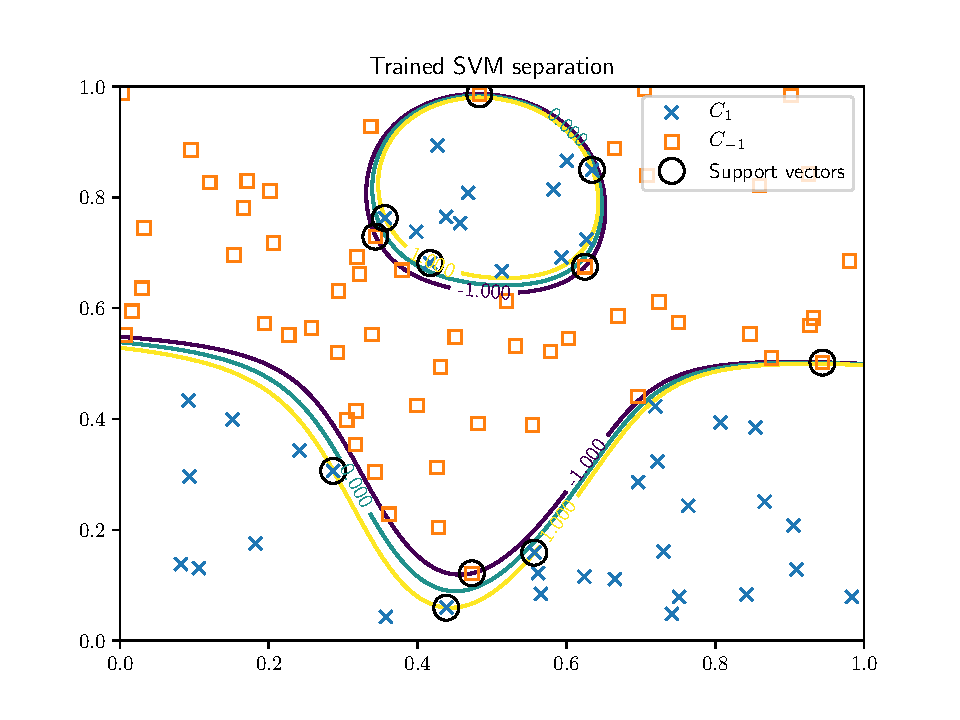
\includegraphics[width=0.7\linewidth]{sep_poly.pdf}
    \caption{Separation obtained with the polynomial kernel SVM}
    \label{sep_poly}
\end{figure}

\begin{figure}[h]
    \centering
    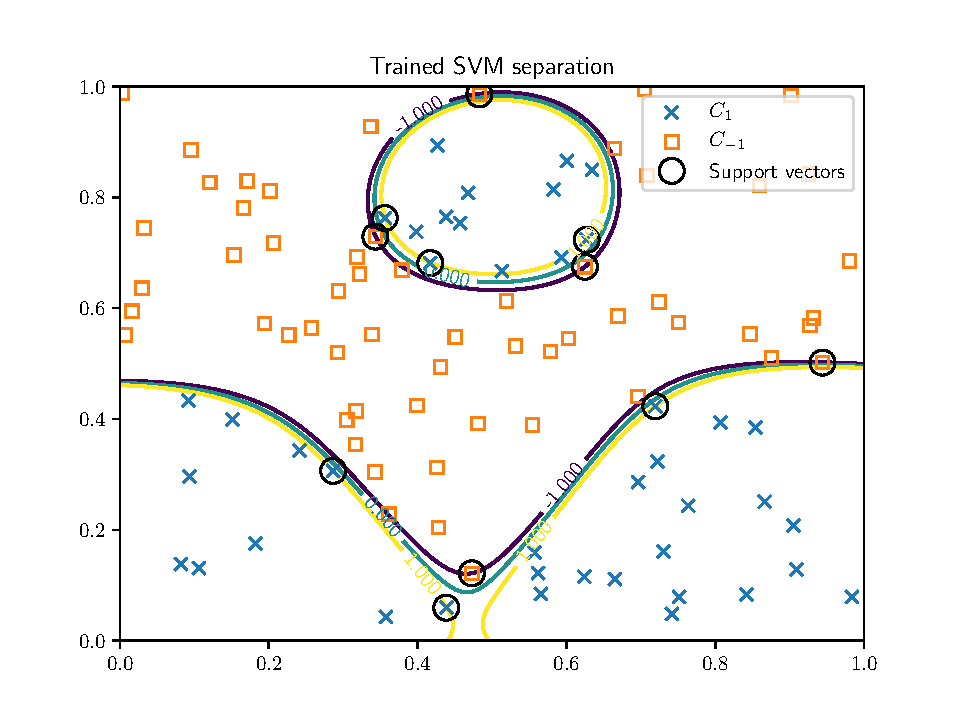
\includegraphics[width=0.7\linewidth]{sep_exp.pdf}
    \caption{Separation obtained with the Gaussian kernel SVM}
    \label{sep_exp}
\end{figure}

The solution based on the polynomial kernel uses the following support vectors:

\begin{itemize}
    \item For $C_1$:
    $$ \left[ \begin{matrix} 0.43857224 \\ 0.0596779 \end{matrix} \right], \left[ \begin{matrix} 0.63440096 \\ 0.84943179 \end{matrix} \right],     \left[ \begin{matrix} 0.48303426 \\ 0.98555979 \end{matrix} \right],     \left[ \begin{matrix} 0.55678519 \\ 0.15895964 \end{matrix} \right],     \left[ \begin{matrix} 0.35591487 \\ 0.76254781 \end{matrix} \right],     \left[ \begin{matrix} 0.28653662 \\ 0.30646975 \end{matrix} \right] $$

    \item For $C_{-1}$:
    $$ \left[ \begin{matrix} 0.34317802 \\ 0.72904971 \end{matrix} \right], \left[ \begin{matrix} 0.94416002 \\ 0.50183668 \end{matrix} \right], \left[ \begin{matrix} 0.48303426 \\ 0.98555979 \end{matrix} \right], \left[ \begin{matrix} 0.6249035 \\ 0.67468905 \end{matrix} \right], \left[ \begin{matrix} 0.472913 \\ 0.12175436 \end{matrix} \right] $$
\end{itemize}

As for the solution based on the Gaussian kernel, the following support vectors were used:

\begin{itemize}
    \item For $C_1$:
    $$ \left[ \begin{matrix} 0.71946897 \\ 0.42310646 \end{matrix} \right], \left[ \begin{matrix} 0.43857224 \\ 0.0596779 \end{matrix} \right],     \left[ \begin{matrix} 0.41702221 \\ 0.68130077 \end{matrix} \right],     \left[ \begin{matrix} 0.62724897 \\ 0.72341636 \end{matrix} \right],     \left[ \begin{matrix} 0.35591487 \\ 0.76254781 \end{matrix} \right],     \left[ \begin{matrix} 0.28653662 \\ 0.30646975 \end{matrix} \right] $$

    \item For $C_{-1}$:
    $$ \left[ \begin{matrix} 0.34317802 \\ 0.72904971 \end{matrix} \right], \left[ \begin{matrix} 0.94416002 \\ 0.50183668 \end{matrix} \right], \left[ \begin{matrix} 0.48303426 \\ 0.98555979 \end{matrix} \right], \left[ \begin{matrix} 0.6249035 \\ 0.67468905 \end{matrix} \right], \left[ \begin{matrix} 0.472913 \\ 0.12175436 \end{matrix} \right] $$
\end{itemize}

\subsection{Complete Python code}

\lstinputlisting[basicstyle=\ttfamily\scriptsize]{hw7.py}

\end{document}